\chapter{Calculation of the AC-Stark-Shift}

The calculation of the \textsc{ac}-Stark-Shift is done, using the formulas resulting from pertubation theory, as carried out in the previous sections. The first part of this chapter reviews the main results regarding the polarizabilities of the ground and first excited state. This will reveal also whether the excited state can also be trapped in the high intensity region of the lasers and how the trapping compares to that of the ground state. All calculations use the computer algebra system mathematica.\\For the meassurement, testing the theoretical foundation, that is presented in this thesis, concrete shift calculations are made regarding the big, crossed dipole trap. At the end of this section, values for the small microtrap will be presented, that will suggest, in how far the goal of imaging atoms in small traps and single sites of optical lattices can be managed. The magnetic field, and thus the quantisation axis is definde to be along the z-direction.

\section{Polarizability}
For the calculation of the polarizabilities for the respective states, the geometry and power of the used laser-beams are not important, since it only depends on the wavelength of the incoming light and on its polarization, that has a notable role for the tensor-polarizability in the vicinity of a transition resonance and renders unimportant, when using very far detuned trap-light. Before talking about concrete results, we recall the formulas given in the theory-section. 
\begin{align}
\alpha=\left[\alpha^0_J+\frac{3m^2_J-J(J+1)}{J(2J-1)}\alpha^2_J\right]\\
\notag\\
\alpha^0_J=&\frac{2}{3(2J+1)}\sum_{K\neq J}\frac{|\braopket{J}{|r|}{K}|^2}{W_K-W_J}\notag\\
\alpha^2_J=&4C\sum_{K\neq J}(-1)^{J+K}\sixj{J}{1}{K}{1}{J}{2}\frac{|\braopket{J}{|r|}{K}|^2}{W_K-W_J}\notag
\end{align}
Following \cite{magic}, the polarizability is calculated using atomic units (a.u.). For the calculation transitions up to $n=7$ were considered. The respective dipole-transition matrix elements are listed below, together with the energy-differences between the levels.

\begin{figure}[H]
\begin{center}
\begin{tabular}{ccc}
Transition&Matrix-element [$\unit{a.u.}$]&Resonance [$\unit{nm}$]\\\hline\hline\\
$2s_{1/2}-2p_{1/2}$&3.3169&670.791\\
$2s_{1/2}-2p_{3/2}$&4.6909&670.776\\
$2s_{1/2}-3p_{1/2}$&0.183&323.2657\\
$2s_{1/2}-3p_{3/2}$&0.259&323.2657\\
$2s_{1/2}-4p_{1/2}$&0.160&274.1203\\
$2s_{1/2}-4p_{3/2}$&0.226&274.1203\\
$2s_{1/2}-5p_{1/2}$&0.1198&256.2312\\
$2s_{1/2}-5p_{3/2}$&0.169&256.2312\\
$2s_{1/2}-6p_{1/2}$&0.0925&247.5061\\
$2s_{1/2}-6p_{3/2}$&0.131&247.5061\\
$2s_{1/2}-7p_{1/2}$&0.0737&242.5426\\
$2s_{1/2}-7p_{3/2}$&0.1042&242.5426\\
$2p_{1/2}-3s_{1/2}$&3.4403&812.645\\
$2p_{1/2}-4s_{1/2}$&0.9167&497.175\\
$2p_{1/2}-5s_{1/2}$&0.4929&427.313\\
$2p_{1/2}-6s_{1/2}$&0.3268&398.554\\
$2p_{1/2}-7s_{1/2}$&0.2397&383.564\\
$2p_{1/2}-3d_{3/2}$&2.2658&610.366\\
$2p_{1/2}-3d_{5/2}$&6.7975&670.776\\
$2p_{1/2}-4d_{3/2}$&0.8627&460.283\\
$2p_{1/2}-4d_{5/2}$&2.5882&460.289\\
$2p_{1/2}-5d_{3/2}$&0.5015&413.262\\
$2p_{1/2}-5d_{5/2}$&1.5045&413.262\\
$2p_{1/2}-6d_{3/2}$&0.3435&391.535\\
$2p_{1/2}-6d_{5/2}$&1.0306&391.535\\
$2p_{1/2}-7d_{3/2}$&0.2565&379.507\\
$2p_{1/2}-7d_{5/2}$&0.7696&379.507\\\\\hline
\end{tabular}
\end{center}
\caption{Reduced Dipole-Transition-Matrix-Elements \cite{magic01} in a.u. and the respective detuning \cite{NIST_ASD}, i.e. the resonance-energy for the relevant levels: $1s_22s_{1/2}$ and $1s_22p_{3/2}$}
\label{matrixelements}
\end{figure}
Figure \ref{alphages} shows how the polarizability behaves for different levels and different wavelength of the incoming laser-light. In this case, $\pi$-polarized light is assumed. The qualitative behaviour does not change due to different polarizations, only the magnitute of the tensor polarizability. The differences in the practical case of our experiment will be discussed later on.
\begin{figure}[H]
\centering
\begin{subfigure}[b]{0.4\textwidth}
                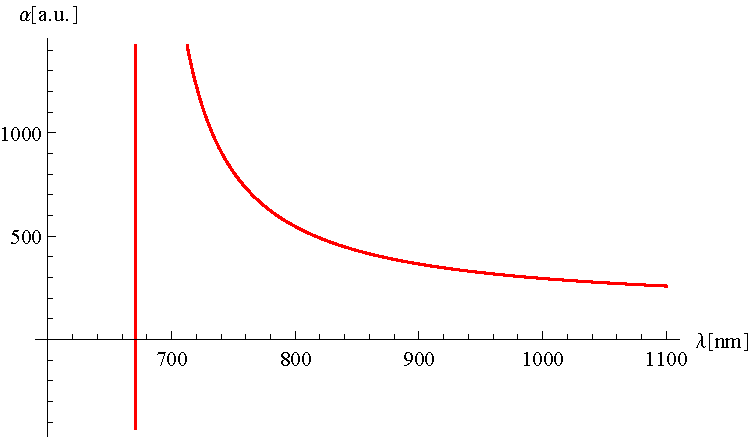
\includegraphics[width=\textwidth]{alphaground}
                \caption{$1s2s_{1/2}$}
\end{subfigure}
\begin{subfigure}[b]{0.4\textwidth}
               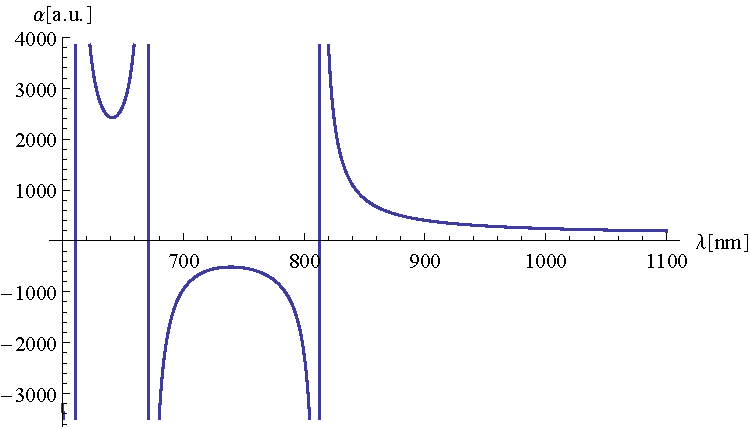
\includegraphics[width=\textwidth]{alphaexited12}
                \caption{$1s2p_{3/2}, |m_j|=1/2$}
\end{subfigure}
\begin{subfigure}[b]{0.4\textwidth}
               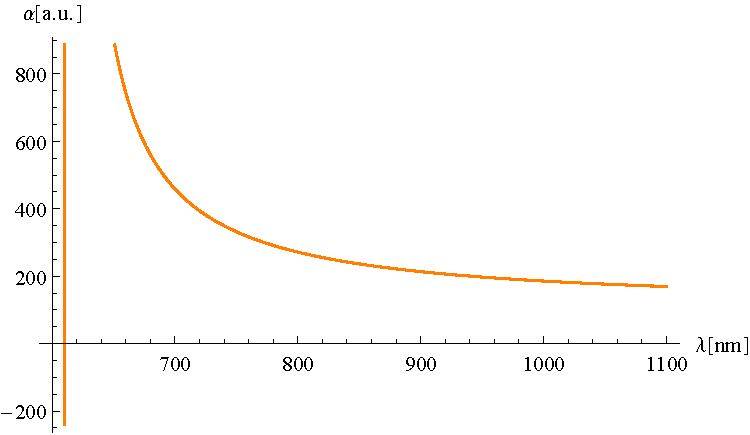
\includegraphics[width=\textwidth]{alphaexited32}
                \caption{$1s2p_{3/2}, |m_j|=3/2$}
\end{subfigure}
\begin{subfigure}[b]{0.4\textwidth}
                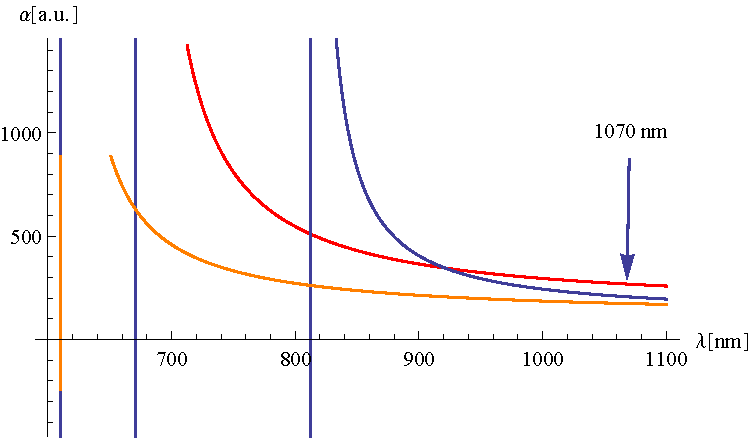
\includegraphics[width=\textwidth]{alphaalltogether}
                \caption{Comparison}
\end{subfigure}




\caption{Polarizability \alpha for the states $1s2s_{1/2}$ (red) , $1s2p_{3/2}, |m_j|=1/2$ (blue) and  $1s2p_{3/2}, |m_j|=3/2$ (orange)}
\label{alphages}
\end{figure}
What can be seen in the plots are some interesting properties. The first important result is, that, considering a far detuned light-source, the ground state, as well as the excited state show positive polarizabilities. This fundamentally contradicts the picture of a two-level system, for example described in \cite{cohen}. In this model, the excited state will be shifted in opposition to the ground state, i.e. the relative sign in the polarizability flips. This reflects the fact, that in a real atom, aspecially in the exited states of Lithium, the structure is much more complicated, than what results from the two-level approximation, because many different levels are roughly in the same energy-range and no single transtion dominates. Practically this results in the fact, that both the ground-state and the first excited states can be trapped in the same type of dipole-trap, because the positive polarizability results in a negative potential. Therefore the atoms are attracted to the highest intensity of the laser-beam. The difference lies in the exact values. For farly detuned light, i.e. above around 1000 nm of wavelength, the ground state shows a higher polarizability, than both excited states, which means, that the potential is deeper for the ground state. From figure \label{relativealpha) can be seen, how the different excited states behave relative to the ground state for the both relevant laser-wavelength for the big and the small dipole-trap in the experiment. As one could expect the difference in the regime of farly detuned light is negligible.

\begin{figure}[h]
\begin{center}
\begin{tabular}{ccc}
State&$\alpha$ at $1070\unit{nm}$ [$\unit{\alpha_{ground}}$]&$\alpha$ at $1064\unit{nm}$ [$\unit{\alpha_{ground}}$] [$\unit{nm}$]\\\hline\hline\\
$1s2p_{3/2}, |m_j|=1/2$&0.7694&0.7726\\
$1s2p_{3/2}, |m_j|=3/2$&0.6487&0.6472\\
\\\hline
\end{tabular}
\end{center}
\caption{Polarizabilities of the excited states for the relevant laser-wavelengths, in relation to the ground state polarizability.}
\label{relativealpha}
\end{figure}

The picture looks different, when cosidering higher frequencies. There, the picture looks different, aspecially when comparing the two excited states with different magnetic quantum number. Below around 900 nm and $m_j=3/2$ the absolute value of the polarizability is much higher than for both other states. Mathematically this can easiest be seen, when looking at the formula for the total polarizability. The tensor-part of this formula is multiplied by a factor, that is -1 or +1, depending on whether $|m_j|=1/2$ or $|m_j|=3/2$. This means, that it decides whether the tensor part is added or subtracted, when calculating the total value. If it is substracted, as for $|m_j|=3/2$ in the vicinity of many resonances the diverging terms will cancel each other out and instead of a singularity, a finite value is the result and the absolute value is smaller.
